%\subsection{Workflow}
\label{sec:workflow}
% Gernot suggests that we must consider entire system
% Hank quantifies that one must consider complex tradeoff space in energy management as hardware is nolonger simply race-to-halt friendly -- race-to-halt, pace-to-idle, optimal and no-idle -- due to changes in the dynamic and static components of energy consumption driven by differences in CMOS and SRAM composition and usage in processors.
% Building on prior work Chou suggests that latency sensitive workloads are different and matter
% Brooks suggest that optimal energy management will require workload specific specialization

% Building on the above observations we uniquely  study performance and energy  impact of slowing down both processors and delaying request processing on network driven workloads from an OS perspective.  Ultimately with the goal of revealing explaining current behavior and guiding future work in both OS and hardware.  

% Using our OS knowledge and prior architectural and application oriented work on power management, we construct a simplified request processing model, that can be expressed mathematically.  We construct the model to reflect what  we believe to be the important interactions that the OS can have on the realized performance and energy when running various types of network oriented workloads.   Specifically,  the model lets us evaluate how slowing down processing and interrupt detection interacts with  variations in the instructions components of OS and Application request processing, the impact of specializing the OS for a single network application, the use of interrupts versus polling and interactions with the use of hardware sleep-states.  Using the model we can predict the general behavior one might observed with respect to both performance and energy.

% We conduct an exhaustive study that sweeps processor slow downs and interrupt delays in the context of four network benchmarks designed to stress different OS and application behaviours.  We evaluate both a general purpose OS and a library OS specialized for to run single network oriented servers.  Doing so lets us vary OS path lengths and efficiencies, differences in interrupt and polling behaviors along with sleep state strategies.

% We then analyze the data to draw validate core observations of how the OS affects the observed combination of performance and energy for the workloads.  We also use the data to evaluate our model.

% model 
% exhaustive search - interesting points
% model seems to match data
% model and data exposes oppunities and shows value of specializain 
% as advocated by brooks furthur suggest a path via OS specialization that can yield novel performance and energy regiemes 
% model enables others to validate 
% model allows both os and hardware designers to evaluate and guide changes
% model 

%https://lucid.app/lucidchart/fc20f7aa-529f-44e7-b9b5-8ed52952f7d5/edit?page=l0EzjAKrzgiu#
\begin{figure}
\centering
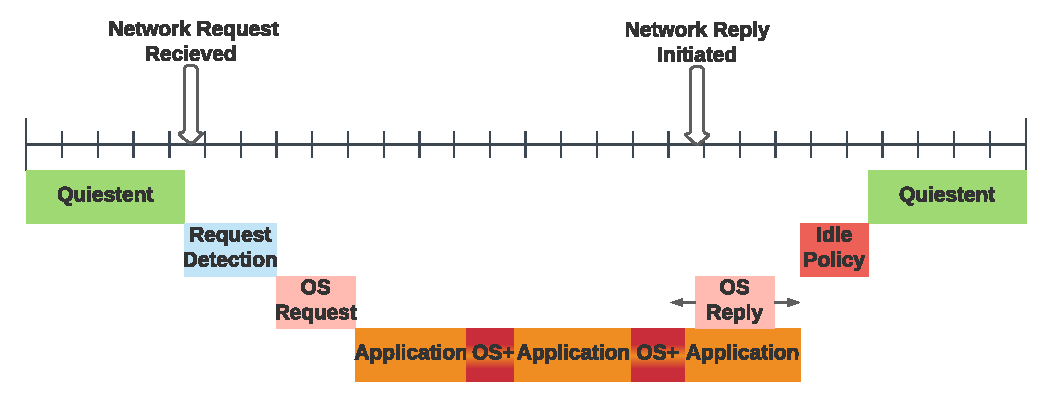
\includegraphics[width=1.1\columnwidth]{figures/timeline_chart}
\vspace*{-10mm}
\caption[]{Application processing request timeline.}
\label{fig:timeline}
\vspace{-0.20in}
\end{figure}

From an OS perspective we break down network driven processing into stages that allows us to organize and reflect the OS and application interaction with the workload request timeline. This break down is illustrated in figure~\ref{fig:timeline}\footnote{Although drawn and discussed from the perspective of a single core, our analysis and evaluation assumes that multiple core could be used to shorten servicing times.}.
% TODO
% We believe the important aspects of OS/network loads are shown in figure 1
% abstraction 
% how we came up with this, to tease apart the interactions
%\textbf{TODO:General nature of the timeline graph across system and network hardware}  

\subsection{Quiescent}
\label{sec:workflow:Quiescent}
Given the packet and transactional nature of network driven services, a quiescent period, in which no requests are present at the server, precedes activity on the server. 

The nature of the workloads drive the length of quiescent period and of course the nature of the work required to service the request (the additional components of the diagram that will be discussed next).  Network services tends to fall into two broad categories Open and Closed Loop.   

\subsubsection{Open Loop:}
\label{sec:workflow:openloop}
In an open loop scenario like a Memcached workload, the external request rate induces an inter-arrival gap that will drive the quiescent period -- longer at lighter loads (lower queries per second (QPS)) and shorter at heavier loads (higher QPS). The arrival rate can largely be considered independent of the time required to service a request. Moreover, providers often set a Service-level Agreement (SLA) target, such as some percentage of requests to be completed under a stringent time budget. There have also been a wealth of research in using these SLA headrooms to lower datacenter energy use mainly by decreasing processor frequencies~\cite{Dynamo, SmoothOperator, oldi-pegasus, adrenaline, heracles, energyproportion, warehouse-power}.
% others have noted this is ripe to explore the trade-offs
%, therefore categorizing system performance into acceptable and unacceptable
%System performance is typically evaluated in terms of the 99\% tail latency it achieves.  
%such as a 99\% tail latency of 500${\mu}$s
%Many interesting interactions and trade-offs exist in Open Loop workloads to affect the latency below the SLA targets and the energy consumed. 

\subsubsection{Closed Loop:}
\label{sec:workflow:closed_loop}
Examples of closed loop workloads are snapshotting a database to a remote server, video streaming or a middle tier service within a data center~\cite{Barroso:2009:DCI:1643608, oldi-study, oldi-pegasus, warehouse-power, energyproportion, WebSearch}.  The work to be done is a sequence of requests that have an inter-dependency on each other. Specifically, the arrival of the next request depends on how fast it takes to service the current request. From a server's perspective, the quiescent period will be bounded by time to transmit both the request and the reply, as well as the time on the client to generate the next request.  
In the closed loop setting, one would like the server to complete every request quickly so that the overall time to complete a task is minimized. However, we find that depending on the nature of the workload and the quiescent period, composed of the network transmission times and client servicing time, there still exist interesting opportunities explore energy-performance trade-offs.
% polling in nodejs/netpipe - edp
% heavy computation vs light computation
% msg size differences
% itr delay -> edp

%However, the quiescent period is bounded by the network round trip time, that depends on  the size of a request and reply packets, and the remote processing time. System performance is largely evaluated on how fast a server can complete the entire task given a network link speed and a remote system.  Given workload specific characteristics such as the processing required and round-trip costs it is possible, as we will see, to find configurations in which the OS interacts with slowing down to improve both time and energy. 

%We know from previous research in energy proportionality in datacenters, the nature of web-centric applications causes diurnal troughs~\cite{Barroso:2009:DCI:1643608, oldi-study, oldi-pegasus, warehouse-power, energyproportion, WebSearch}, and one method with which to increase energy efficiency during these troughs is to increase performance. We find even in the performance driven closed loop applications, there still exist interesting trade-offs between OSes.

%Given our goal of studying and explaining the implications of the OS on network driven processing our analysis framework, and evaluation, includes closed loop settings.  In particular, we use a simple ping-pong application to stress OS behavior while varying packet-sizes to reveal how OS path length and path efficiency interacts with slowing down processing, relative to the round trip time observed at the server.  Additionally we use a second closed loop that stresses single core application processing with negligible packet sizes to evaluate if OS structure can impact the application efficiency.  

% Often research tends to categorize close loop settings as either not representative of cloud computing or imply that energy-performance tradeoffs are not interesting due to the hight utilization closed-loop processing can imply.  
\subsection{OS Request Detection}
Fundamental to any operating system is how it detects and schedules processing in response to IO device activity.  At the two extremes are interrupt and poll driven detection.  

\subsubsection{Interrupt driven IO}
\label{sec:workflow:interruptio}
Using interrupts has three important implications: 1) it can be used to wake a processor from a halted state, which the OS entered to sleep the processor (c-states), in response to external activity, 2) allow an OS to arbitrate processing across competitive devices in a multi-programmed/multi-device setting, 3) interrupts have inherent performance costs associated with it --  latency in starting to handle a request, either because of the costs associated with preempting work~\cite{whenpollisbetter} or c-state exit penalties\cite{cpuidle_policy}. Interrupts can also have a negative impact on the instruction efficiency, such as Instructions Per Cycle (IPC), due to induced micro-architecture hazards such as the inability to pre-fetch or speculatively execute across an interrupt.
%% brings in angle of energy and performance

\subsubsection{Poll driven IO}
%todo: modify to ack use of halt on cache line in stead of just polling.  
\label{sec:workflow:pollio}
Most modern NICs devices expose a cache-friendly interface that permits the processors to read a per-core memory address to determine if the device has received data that requires processing by the core.  This allows software to directly poll the device and initiate software handling without an interrupt.  This approach reduces latency and other performance penalties associated with interrupt driven IO but requires a busy CPU. In the extreme, a customized OS path supporting a single application can run a poll loop on every core to constantly check for work, conduct the work and then go back to polling for new work and thus never halting the processors \footnote{It is worth noting processors also have the ability to halt in a way that an update to a cache line will awaken it, there exists the possibility of implementing the poll in combination with sleep states. We do not explore this possibility, leaving it for future work.}.

%However, the period in which the device is checked requires CPU activity and thus limits the ability to halt the cores when there is no work to be done.

%Kim et al.\cite{pacingtoidle}, referred to a regime in which one keeps the processor busy as 'no-idle', an alternative energy management strategy. In the context of network driven processing we will refer to this as an aggressive polling or simply polling strategy.  In general, such an aggressive poll approach is assumed to maximize performance by avoiding interrupt overheads and minimize latency at a cost to increased energy use. 

\subsubsection{Hybrid driven IO}
\label{sec:workflow:hybridio}
% https://wiki.linuxfoundation.org/networking/napi
A general purpose OS typically exploits some form of hybrid IO strategy alternating between interrupts and polling when servicing high speed NICs. A common strategy is to use interrupts when the load is low and switch to polling when load is high and back to interrupts when load reduces.  A general purpose OS, even under sustained high load, bounds the poll phase to avoid the starving other devices and software. Linux's New API (NAPI)\cite{NAPI} framework implements this hybrid scheme.
%% these ideas help to explain the vertical of slowing down proceessor on Linux netpipe, memcached at really low QPS

%% Han - not sure we need to examine it in this detail, seems like re-explanation of the paragraph above, think NAPI and its implementation is already well known
%The first arrival of a packet generates an interrupt which switches the servicing of the device to polling if some threshold of packets are present.  If the number of packets drop below the threshold when the device is polled or a time limit for poll is exceeded the device will no longer be polled and interrupts re-enabled in order to detect activity on the NIC.  
%The NAPI framework, in addition to NIC processing budgets,  supports prioritization across devices. 
% In Linux the NAPI polls are processed via softirqs.  Checks for and processing of softirqs happens when ever the system returns to userspace or a hardware interrupt exits.

Specializing an OS to support the execution of a single application can explore more extreme strategies like the aggressive polling, described above, given that it need not arbitrate the device or cores and can be programmed and integrated with a single application.  
%% a general purpose must not starve out vs specialized os

\subsubsection{Interrupt Delaying}
\label{sec:workflow:itrdelay}
%\tikzstyle{startstop} = [rectangle, rounded corners, minimum width=3cm, minimum height=1cm,text centered, draw=black, fill=red!30]
\tikzstyle{io} = [trapezium, trapezium left angle=70, trapezium right angle=110, minimum width=3cm, minimum height=1cm, text centered, draw=black, fill=blue!30]
\tikzstyle{process} = [rectangle, minimum width=3cm, minimum height=1cm, text width=2cm, text centered, draw=black, fill=orange!30]
\tikzstyle{decision} = [diamond, minimum width=3cm, minimum height=1cm, text width=1cm, text centered, draw=black, fill=green!30]
\tikzstyle{arrow} = [thick,->,>=stealth]

%\begin{figure}
\centering
%\resizebox{5cm}{3cm}{%
\begin{tikzpicture}[node distance=2cm]

\node (start) [startstop] {ITR=\textit{n} $\mu$s};
\node (dec1) [decision, below of=start] {ITR==\textit{0}?};
\node (pro1) [process, right of=dec1, xshift=1.5cm] {ITR-=\textit{2} $\mu$s};
\node (dec2) [decision, below of=dec1, yshift=-0.5cm] {RX/TX Event?};
\node (pro2) [startstop, left of=dec2, yshift=1.5cm, xshift=-0.8cm] {Assert Interrupt};

\draw [arrow] (start) -- node[anchor=west] {check} (dec1);
\draw [arrow] (dec1) -- node[anchor=north] {no} (pro1);
\draw [arrow] (pro1) |- node[anchor=west] {update} (start);
\draw [arrow] (dec1) -- node[anchor=west] {yes} (dec2);
\draw [arrow] (dec2) edge[loop right]node{no} (dec2);
\draw [arrow] (dec2) -- node[anchor=east] {yes} (pro2);
%\draw [arrow] (pro2) -| node {} (start);
\draw [arrow] (pro2) |- node[anchor=east] {reset} (start);
\end{tikzpicture}
%}
%\vspace*{-5mm}
%\caption{ITR-Delay algorithm flowchart.}
%\label{fig:itr_delay_flowchart}
%\vspace{-.25in}
%\end{figure}
%We flowchart the algorithm from the NIC's datasheet~\cite{82599} in  Figure~\ref{fig:itr_delay_flowchart}
A common feature of modern high speed NICs is the ability to delay the delivery of interrupt when an event such as packet arrival or transmission completion. By manipulating this setting, software can limit the minimum time between interrupts or in other words the maximum rate at which the NIC events can interrupt the CPUs. The NIC used in this study exposes this mechanism via an Interrupt Throttling (ITR) setting. Software uses the ITR register to configure a delay in 2$\mu$s increments.  If the spacing of events, such as packet reception, is less than  $2{\mu}s \times ITR$ the NIC will delay assertion.  If on the other hand events are sufficiently separated an interrupt will be asserted immediately.   

By default the Linux device driver attempts to automatically set this interrupt delay value to reduce interrupt overheads.  We disable this feature and manually control its value to explore the impact of delaying interrupts on performance and energy. Delaying interrupt detection introduces an additional OS control mechanism. For example, delaying a interrupt can induce prolonged quiescence periods, in which processor idle policies can take advantage of.

%Combining interrupt driven IO and delaying interrupt assertion via ITR setting, we can explore the impact of delaying packet detection and thus delaying processing of requests.

%Depending of the state of the processor the NIC can buffer packets in its own memory or on the main memory of the host\footnote{According to the data sheet if the processor is in sleep state packets can only be buffered on the card's limited memory and once exhausted packets will be dropped}.  

%% TODO: may move down

\subsection{OS Request Processing}
\label{sec:workflow:osreqproc}

Once the OS detection mechanism identifies that the NIC has data to process, several components of OS functionality must be run in accordance with the execution model of the OS. Specifically, the OS's network stack parses the received packet's layer 2 frames, TCP/IP headers and eventually to the application layer for processing. %% TODO shorten

%%Specifically, device driver code must dequeue layer 2 frames and schedule them for processing by the appropriate network protocol code. This code must ultimately determine the application end point, a port in the case of IP and TCP, and enqueue, the encapsulated data, for application processing. 

This work on a general purpose OS is typically split between two levels of scheduling; 1) interrupt level in which minimal work is done but at the highest critical priority and is run to completion (typically called the top-half processing), 2) the so-called bottom-half uses various kernel facilities to execute both device driver logic and protocol processing in a manner that can be preempted and rate limited.  Regardless, all this work is done at the OS privilege domain and ultimately prepares data for application processing (pre-emptable) and is independently scheduled at lower privilege and priority. %% contrasted with specialized os

An application specific library OS stack shed much of the above complexity, both shortening the path and eliminating the above privilege scheduling domains~\cite{arrakis,ix,EbbRT}. It can exploit short-cuts that allow run to completion execution of all the logic, including application processing in response to detecting device activity. As such, the library OS is used to explore the impacts of shorter OS hot-paths.
%customized to running a single network service.  

\subsubsection{Application Processing}
\label{sec:workflow:appproc}

%Once the OS has completed protocol processing it enables application logic to begin.  Depending on the workload this may be very simple as in the case of a workload like memcached or it require significant cpu activity as in the case of  an application server written in managed runtime such as nodejs or one that does non-trivial computational work to service a request. 

As illustrated in figure~\ref{fig:timeline}, during application processing, the OS logic may be interleaved.  This work roughly falls into two categories, synchronous work done in service of this application request (page-faults, system calls, etc) and asynchronous work not having to do with this request (OS background work, processing of other requests or processes). Library OS's can often avoid interleaving asynchronous work, unrelated to the request handling,  and thus minimize jitter and improve IPC. %% application work is fixed typically

\subsubsection{OS Reply Processing}
\label{sec:workflow:osrepproc}

Figure~\ref{fig:timeline} shows that at some point during application processing, a reply is generated and submitted to the OS for transmission.  This can often be handled in an asynchronous fashion depending on the OS semantics;  the OS can initiate protocol processing and device transmission in parallel with the remaining application logic (eg. book keeping, cleanup and preparation for the next request). This overlap reveals a potential opportunity for performance-energy trade-offs. Specifically, it is possible given a particular packet arrival rate that slowing down causes the remaining application work to coincide with the time for the next request to arrive in both a closed and open loop settings, therefore keeping the processor busy. As such it maybe possible that trade-offs in sleep state latency, interrupt overheads and polling leads to better performance at lower energy consumption.  
%Where 

%This potential overlap is an important distinction as it reveals that some applications may have an associated opportunity for a performance/energy optimization.  Specifically, it is possible given a particular arrival rate that there maybe ways of slowing down that permit the remaining application work to overlap with the time for the next request to arrive in both a closed and open loop settings.  As such it maybe possible that trade-offs in sleep state latency, interrupt overheads and polling leads to better performance at lower energy consumption.  

\subsubsection{Idle Policy}
\label{sec:workflow:idlepolicy}

If all processing is complete, and no traffic is pending and aggressive polling is not in use, the OS can use a policy that select a hardware sleep state (c-state) to halt the core to. Various policies around optimizing them have been extensively studied as well~\cite{dynsleep,dreamweaver,slowdownorsleep}. Each sleep state is has an associated reduction in static power consumption. In the extreme, the deepest sleep states can flush micro-architectural state such as caches and power down these structures. However, each sleep state also imposes a progressively larger wake-up latency and potential impact on execution efficiency given the possible flushing of state~\cite{7425206}. %See \cite{brooks,udpm} for more information regarding C-States. 

%If there is space we might want to add the c-state for our processor similar to what was done in Brooks

There is clearly a relationship between the Idle Policy and Request Detection processing.  For a general purpose OS the normative assumption is both are interrupt driven.  Where an inter-dependency between the halt and interrupt mechanisms of the processor is exploited.  

In this study, we allow Linux's scheduler and default idle policy to decide if a core should be halted and to what state.  This policy exploits various statistics to estimate how long the core is likely to be idle. It takes into account an estimate of when the next interrupt will likely occur from any source.  This is a subtle implementation that interacts across many layers of the OS software including the device drivers.  The idle driver framework also includes code provided by the processor manufacturer to evaluate the latency penalties and suggested minimum residency times.  This allows us to see the impacts of making informed decisions regarding sleep states.  

The library OS uses two simple policies: 1) when there is no work to process on a core, the processor is put into the deepest sleep state (C7), thus ignoring any trade-offs in use of other sleep states.  This enables us to focus on the interaction that slowing down the processor and adjusting interrupt delay can have with the fixed use of a deep sleep. The second approach is to use an aggressive pool loop for IO event detection (\cref{sec:workflow:interruptio}) where the processor is kept busy and there is no idle policy. 
%% discussion section later about alternatve sleep state policies

\section{Performance and Energy}
\label{sec:slowdown}
In this section, we discuss how the decomposition of the timeline in figure~\ref{fig:timeline} relates to slowing down processor, delaying requests, and OS specialization for network processing.

\subsection{Interactions with Slowing Down the processor}
\label{sec:workflow:dvfs}

As noted, the use of Dynamic Voltage Frequency Scaling (DVFS) of a processors allows software to adjust the energy consumption of CMOS based logic while trading off the rate at which instructions complete.  As noted by~\cite{slowdownorsleep, 10.1109/40.888701, pacingtoidle, udpm} static or leakage energy consumption (i.e. caches, TLBs) is not particularly affected by DVFS and induces a base cost for keeping a fix core architecture active.\footnote{Opposed to big-little or re-configurable core architectures.}

Our study focuses on revealing how "slowing down" processing, using DVFS, interacts with the processing of network driven software stacks and the resultant energy and performance realized. From this perspective we simply view DVFS as a speed control setting that can dilate CPU processing components of the request timeline in exchange for reduction in energy consumption.

From this perspective, the three obvious components that can be affected are OS Request, Application and OS Reply processing. For any given OS, there will be a hot-path instruction sequence that will be commonly exercised to process the request packets.  The OS implementation will determine the nature of the instructions that will compose this path for a particular workload.  As such, at the fastest DVFS setting there will be a characteristic mean number of cycles that will be required and thus an IPC efficiency realized.  It is important to note that OS IPC does not necessarily imply better or worse performance and energy. What matters more is the net effect the OS instructions have with respect to application efficiency (eg. request processed per OS cycle). %% cite others 

\subsection{Interactions with Delaying Interrupts}
\label{sec:workflow:itr}
Prior work suggests that delaying request processing can interact with DVFS and c-states in latency sensitive workloads to yield useful energy performance trade-offs~\cite{mootaz, udpm}. To this end, we sweep interrupt delay values for all our workloads OS configurations, and DVFS values.

As Mootaz et al.\cite{mootaz} observed in latency focused workloads, the "latency-slack" between the mean time to servicing a request and the SLA target creates an opportunity for energy-performance trade-offs.  In particular, it maybe possible to reduce mean performance by not executing requests as fast as possible and or not processing request immediately upon their arrival to reduce energy consumption while not violating the SLA target.  

Both these prior works suggest an energy management policy that relies on delaying processing of application requests. Both build an application specific prediction model of the time that is required to service requests and take a specification of the required tail latency SLA target. The  controller strategies exploit a combination of delaying processing and slowing down to find an optimal setting that ensures acceptable tail latencies while reducing the energy consumption.  The intuition is that there are advantages to using batching to consolidate idle time, lengthen the time that the processor can be in deeper sleep state and/or savings that come from slowing down processing time given the latency slack.    

We uniquely explore how delaying processing can be enacted by exploiting interrupt delay setting of the NIC. Specifically, we explore the impact of slowing down interrupt delays, controlled by the OS, to see if similar benefits might exist while not assuming particular workload knowledge. In particular, we expect that delaying interrupts can interact with OS code and the inherent packet nature induced by fixed Message Transmission Unit (MTU) constraints. If a request requires several MTU's, then delaying interrupts has the potential to reduce the interrupt overheads. Similarly if there is advantages to batching request, as the prior work has noted, this too could be this OS control.

\subsection{Interaction with Specializing OS Paths} 
\label{sec:workflow:osspec}
% \begin{em}
 Critically we find that optimizing the hot-path of network processing in an OS can lead to valuable energy savings.  
 %If the OS can support the application work in shorter number of cycles using less energy it can lead to an improvement in application IPC and energy efficiency. 

In an OS centric workload, a shorter OS path can allow one to slow down the processor and not impact the application performance.  We find that specialized OS networking paths can have lower IPC, due to the nature of the instruction mix, and thus have performance that is less affected by a lowered processor speed and yet still have the benefit of lowered energy use. In some sense, this is counter to the extreme IPC efficiency that can be had by running loops of NOPs.  The important point is that despite having a lower IPC, more application work such as network processing, is being completed in the same amount of time but consumes less energy (\cref{fig:mcd_detail_1}, \cref{fig:mcd_overview}). Further, this reveals that certain instruction mixes (i.e. non-ALU bound) are not as affected by a slowed processor speed and that OS path length optimizations can exploit this to achieve better energy efficiency. \footnote{Remembering that power is a function of $Voltage^2 \times Frequency$ different instructions can have different energy and time profiles.  This phenomena which we expose is very interesting and requires further study.}

%This uniquely highlights that certain instruction mixes yield behavior, such that as processor speed is changed, their energy consumption goes down due to a drop in voltage and yet do not seem to be affected by processor speed impacts on frequency and that OS paths can exploit this to achieve better efficiency.\

% %% by optimizing OS path, created a path with 2 benefits: 1) get more work done, 2) instructions less sensitive than DVFS, not ALU bound, i.e. memory-bound instructions likely

In the case of a service oriented workload that has significant application computation, such that the fraction of the instructions composed by the OS network processing is small, there is still a potential for improved performance and energy trade-offs.  Customized OS paths can both reduce the time spent in the OS processing and improve the application code IPC (\cref{fig:mcdsilo_detail}) due to a reduction in architectural hazards associated with interrupts, protection domain crossing, etc.  This time reduction, effectively increases the headroom in which the benefits of either slowing down processing and or delaying interrupts can be used to find an optimal setting for the workload (\cref{fig:mcdsilo_overview}). 
% % mcdsilo
% \end{em}   
 
 \subsubsection{Polling can be energy efficient}
 Another less obvious interaction that can occur is between the use of polling versus interrupts and halting.  Given that polling is a CPU operation, it will interact with processor speed settings.  In particular, it can be possible that at a slower processor speed setting, polling can be more energy efficient and effective with respect to the net performance realized. A core finding is that aggressive polling can be combined with slowing down processing to find a setting that yields best case performance at a lower energy consumption for some workloads (~\cref{sec:closed_loop:poll}~\cref{sec:mcd:poll}).   
 %An example is when the workload is closed loop and transmission times are small.  .  

% \begin{em}

% \end{em}

% Netpipe shows best performance and best efficiency is a function packet size and ITR


%\subsection{Application Perspective}
%Figure~\ref{fig:timeline} shows the application is waiting to be woken up to process new packets (a). Next, an interrupt (b) is fired and the OS network stack begins processing the received packet (c). The application level work begins, alongside there are also interspersed OS work which may or may not be in direct support of application(d). The tail end of the application work (e) typically entails a response packet being sent, the period of time with which the response packet is physically sent can proceed in parallel with the rest of the application level work. The end of every request handling (f) also revolves a set of OS policies to decide the next state of the software and hardware. Work is time spent executing instructions required to service a request, it is a function of the software, hardware, and workload itself. Whereas, idle time is a function of arrival rate of packets.
%
%\subsection{Hardware Perspective}
%Slowing down of the processor causes an increase in the time spent in portions of application and OS work while reducing energy use. Slowing down of interrupt delays contributes to the increase of time spent in the idle states, the longer a processor idles the more energy it can save.
%
%\subsection{OS Perspective}
%OSes overall behaviour is a function of how it behaves during both the working and idle portions of time, there also exists a clear inter-relationship between the two. 
%
%The amount of energy used during this idle period is dependent upon the OS idling policies; in terms of which level of idle state is selected.
%
%\subsection{Equations}
\label{sec:model}

\begin{figure}
\centering
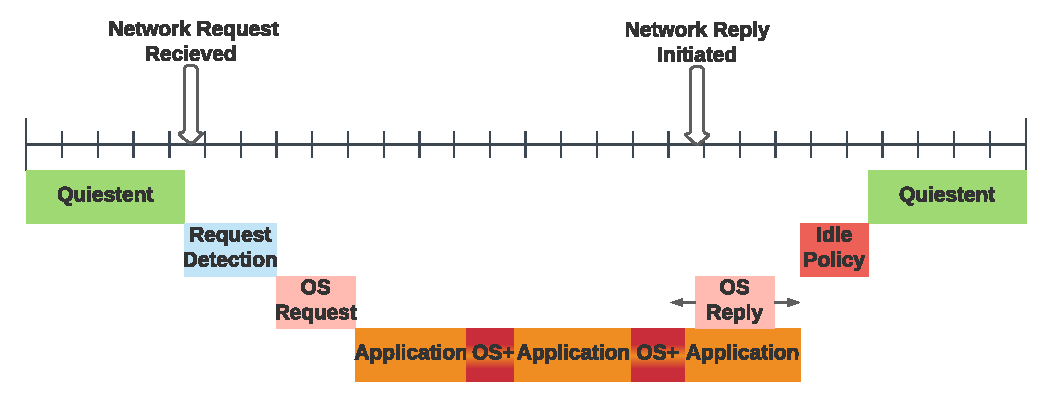
\includegraphics[width=0.5\textwidth]{figures/timeline_chart}
\caption[]{Logical execution timeline for a single application request}
\label{fig:timeline}
\end{figure}

\subsection{Equations}

Using the timeline show in figure X, the total time between two consecutive requests arriving at an arrival rate can be modeled as:

$\delta t = t_{\text{detect}} + t_{\text{osref}} + t_{\text{app}} + t_{\text{idlepolicy}} + t_q$

where 

$\delta t = $ time between the arrivals of two consecutive requests

$t_{\text{detect}} = $

$t_{\text{osref}} = $

$t_{\text{app}} = $

$t_{\text{idlepolicy}} = $

$t_q = $

For a constant arrival rate and ignoring stochastic effects for a qualitative analysis, $\delta t = \frac{1}{\lambda}$ where $\lambda$ is the arrival rate. So,

$\delta t = t_{\text{detect}} + t_{\text{osref}} + t_{\text{app}} + t_{\text{idlepolicy}} + t_q = \frac{1}{\lambda}$

This implies that the quiescent time is:

$t_q = \left[\frac{1}{\lambda} - t_\text{busy}\right]^+$

where $t_{\text{busy}} \equiv t_{\text{detect}} + t_{\text{osref}} + t_{\text{app}} + t_{\text{idlepolicy}}$

and 

$[x]^+ = \max(x,0)$

i.e. $[x]^+$ is the positive part of $x$.

In other words, if the arrival rate $\lambda$ is small, there is an opportunity for the processor to enter a quiescent state ($t_q > 0$) but as the arrival rate increases, the time processing the request, $t_\text{busy}$ exceeds the inter-arrival gap leading to requests accumulating in the queue. 

This relationship also applies to the closed-loop case (Netpipe and NodeJS) with the additional constraint that the arrival rate and thus the inter-arrival gap is no longer independent of $t_\text{busy}$.

We will generally work in the regime where $t_q \geq 0$ i.e. the arrival rate is small enough that there is some opportunity to sleep if sleep states are enabled.

Given this time decomposition, one can compute the total energy consumed for each request as follows:

$E = P_\text{detect} t_{\text{detect}} + P_{\text{work}} \left[t_{\text{osref}} + t_{\text{app}} + t_{\text{idlepolicy}}\right] + P_q t_q$

where three different power regimes have been introduced:

$P_\text{detect} = $

$P_\text{work} = $

$P_q = $

We can now posit the dependence of some of the terms on DVFS.

Suppose the workload needs $N_i$ instructions. One would expect $t_\text{app}$ to scale as:

$t_{\text{app}} \propto \frac{N_i}{f}$

where $f = $ CPU frequency. Of course, there might be deviations from this behavior and one can posit a power law dependence as:

$t_{\text{app}} = A\frac{N_i}{f^{1+\alpha'}}$

where A is a constant of proportionality and $\alpha'$ is an arbitrary parameter. $\alpha'$ = 0 would fit the baseline case where time scales inversely with frequency.

Since we control DVFS and not frequency directly, we can change this to

$t_{\text{app}} = A\frac{N_i}{\Delta^{1+\alpha}}$

where DVFS = the chosen DVFS value and $\alpha$ is some scaling power that can be inferred from data. The other time values don't depend on DVFS.

The total energy consumed depends on various power values which in turn can depend on DVFS. Here, we posit that $P_{\text{work}}$ has a power law dependence on DVFS. To motivate this, the power consumed by a processor scales as:

$P \propto V^2 f$

where V = the operating voltage and f = CPU frequency. DVFS scales both voltage and frequency but not necessarily in a linear way. The general power law assumption is parameterized by a second parameter, $beta$, as follows:

$P_{\text{work}} = B \Delta^{2+\beta}$

where B is a constant of proportionality and $\beta$ can be unrestricited and is meant to be inferred from the data. Depending on the exact setup, it is possible that $P_{\text{detect}}$ also scales with DVFS and in that case, we will set $P_{\text{detect}} = P_{\text{work}}$.

At a qualitative level, the two relationships,

$\boxed{\delta t = t_{\text{detect}} + t_{\text{osref}} + t_{\text{app}} + t_{\text{idlepolicy}} + t_q}$

$\boxed{E = P_\text{detect} t_{\text{detect}} + P_{\text{work}} \left[t_{\text{osref}} + t_{\text{app}} + t_{\text{idlepolicy}}\right] + P_q t_q}$

with the requirements that:

$\delta t = \frac{1}{\lambda}$ or equivalently, $t_q = \left[\frac{1}{\lambda} - t_\text{busy}\right]^+$ with $t_{\text{busy}} \equiv t_{\text{detect}} + t_{\text{osref}} + t_{\text{app}} + t_{\text{idlepolicy}}$.

can be used to plot the behavior of energy consumed vs time (latency, total run-time) for various values of $\alpha$ and $\beta$.

%\subsection{ITR-Delay algorithm}

%\subsection{ITR-Delay algorithm}
